% !TEX program = xelatex
\documentclass[
  10pt,
  twoside,
  openany,
  b5paper, % 以上均为 ctexbook 提供的文类选项
  colorscheme = basic, % 请根据需要选择或定制配色方案
]{qyxf-book}
\usepackage{pdfpages}
\usepackage[contents = 钱院学辅, scale = 15, color = black, angle = 50, opacity = .10]{background}
\includepdfset{pagecommand={\thispagestyle{plain}}}

\title{分子细胞生物学笔记}
\subtitle{Notes on Molecular Cell Biology}  % 可选
\author{越杰91骆华玥}
\date{2021 年 2 月 3 日}
%\typo{AlphaGo}  % 排版人员信息,选填

% 定制元信息
\org{\Large\textit{钱学森书院学业辅导中心}\\\textsc{Qian Xuesen College Academic Counseling Center}}
\footorg{\textsc{Qian Yuan Xue Fu}}
\cover{
	\begin{tikzpicture}[remember picture, overlay]
		\begin{pgfonlayer}{background}
			\node at ($(current page.east)+(0in,0in)$){
				
\includegraphics[width=.8\textwidth]{cover.png} };
		\end{pgfonlayer}
	\end{tikzpicture}
}
\license{}  % 清空许可证信息

% 调整封面标题大小
\renewcommand{\titlefont}{\Huge\bfseries}
\renewcommand{\subtitlefont}{\LARGE\itshape}

\begin{document}

\maketitle

\chapter*{前言}
\thispagestyle{empty}

由于上课老师的PPT及课本中均有许多是考试不涉及的,故笔者复习时自己按照课本《分子细胞生物学》和PPT中内容手写整理出这份复习资料。这份复习资料笔者于考试前一天整理完,考试当天上午又复习一遍,下午考试,发现考试内容绝大部分均有覆盖到。考试内容几乎全部是基于课本的最基础的东西。由于目前没有任何一个学府或组织出有生物复习资料,同学们复习考试又十分需要,笔者在此分享出自己整理的这份资料,希望对大家有所帮助,在其帮助下能考到满意的成绩。

\rightline{——越杰91\ 骆华玥} 
\newpage
\setcounter{page}{1}

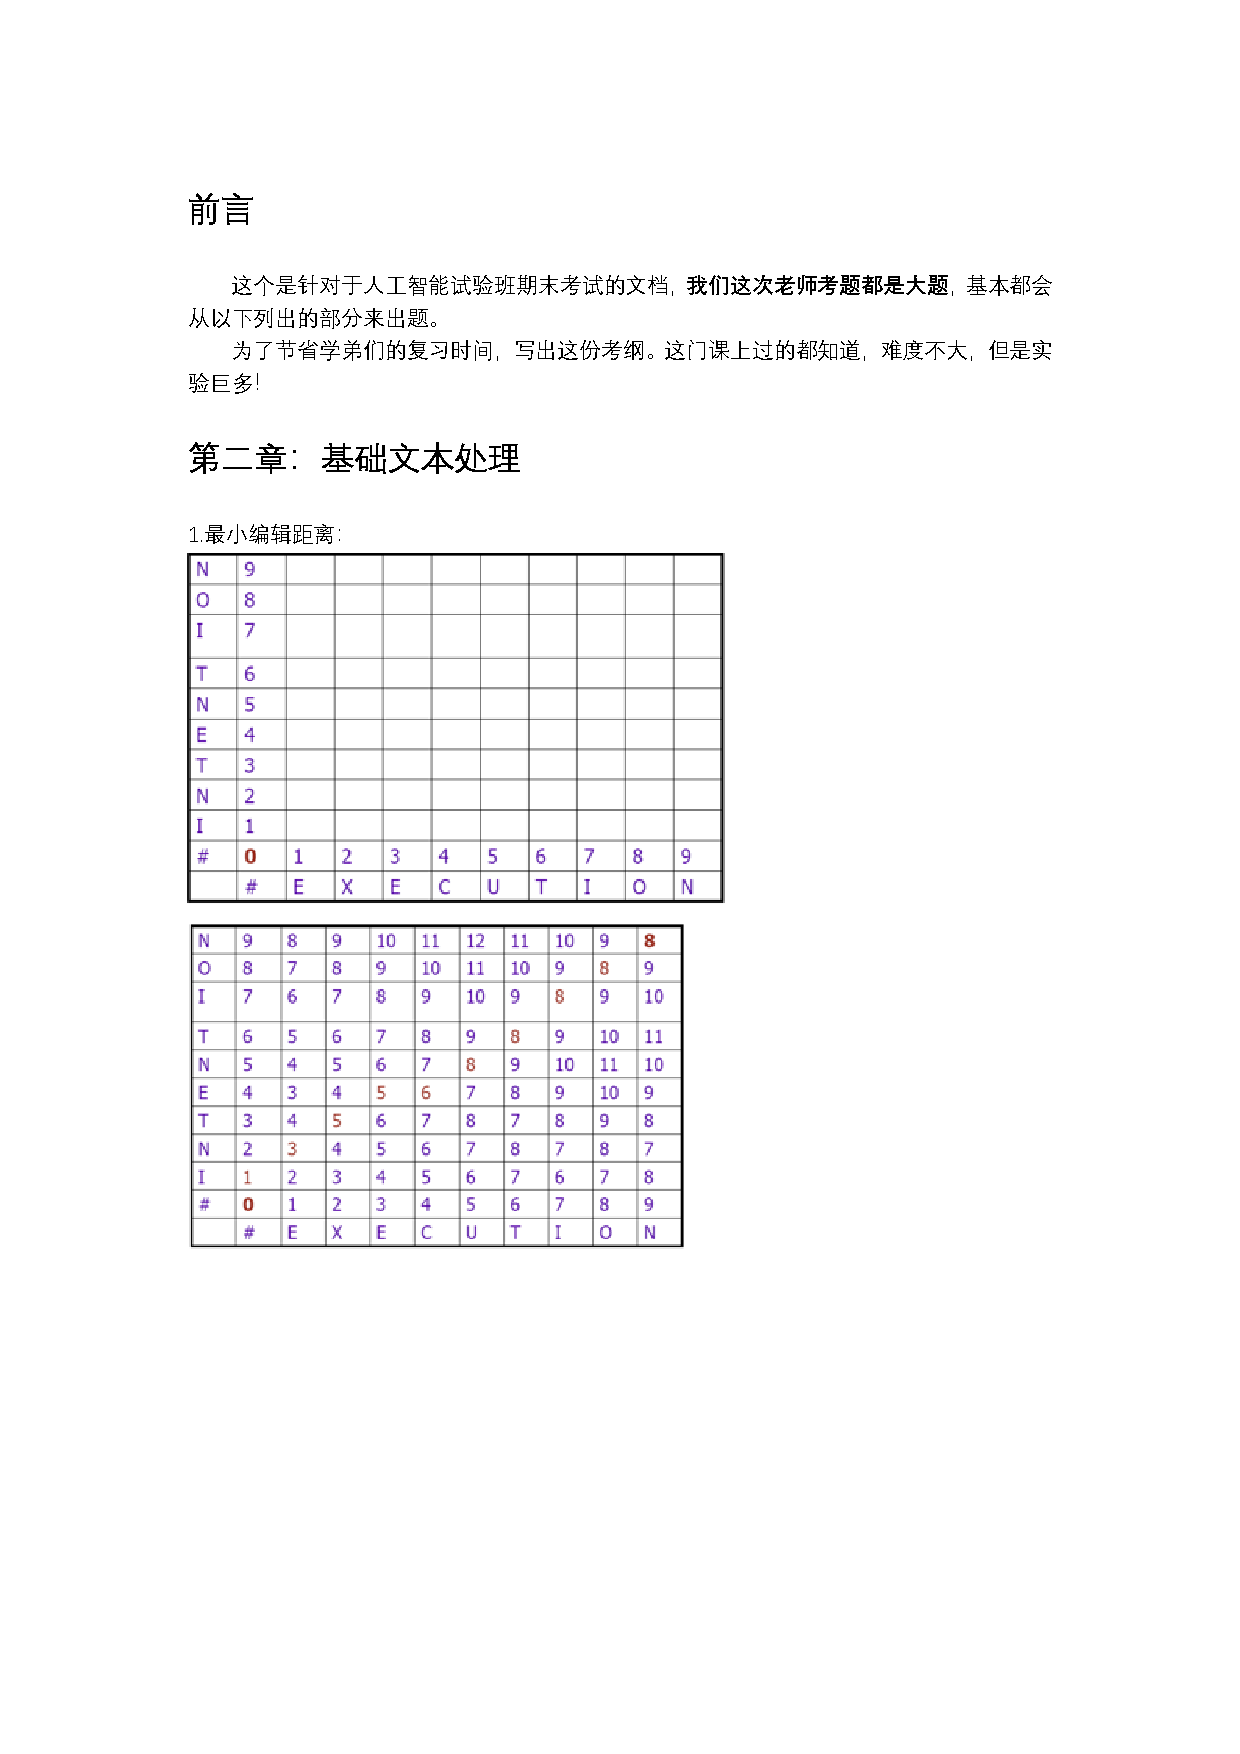
\includepdf[pages = - ]{content.pdf}

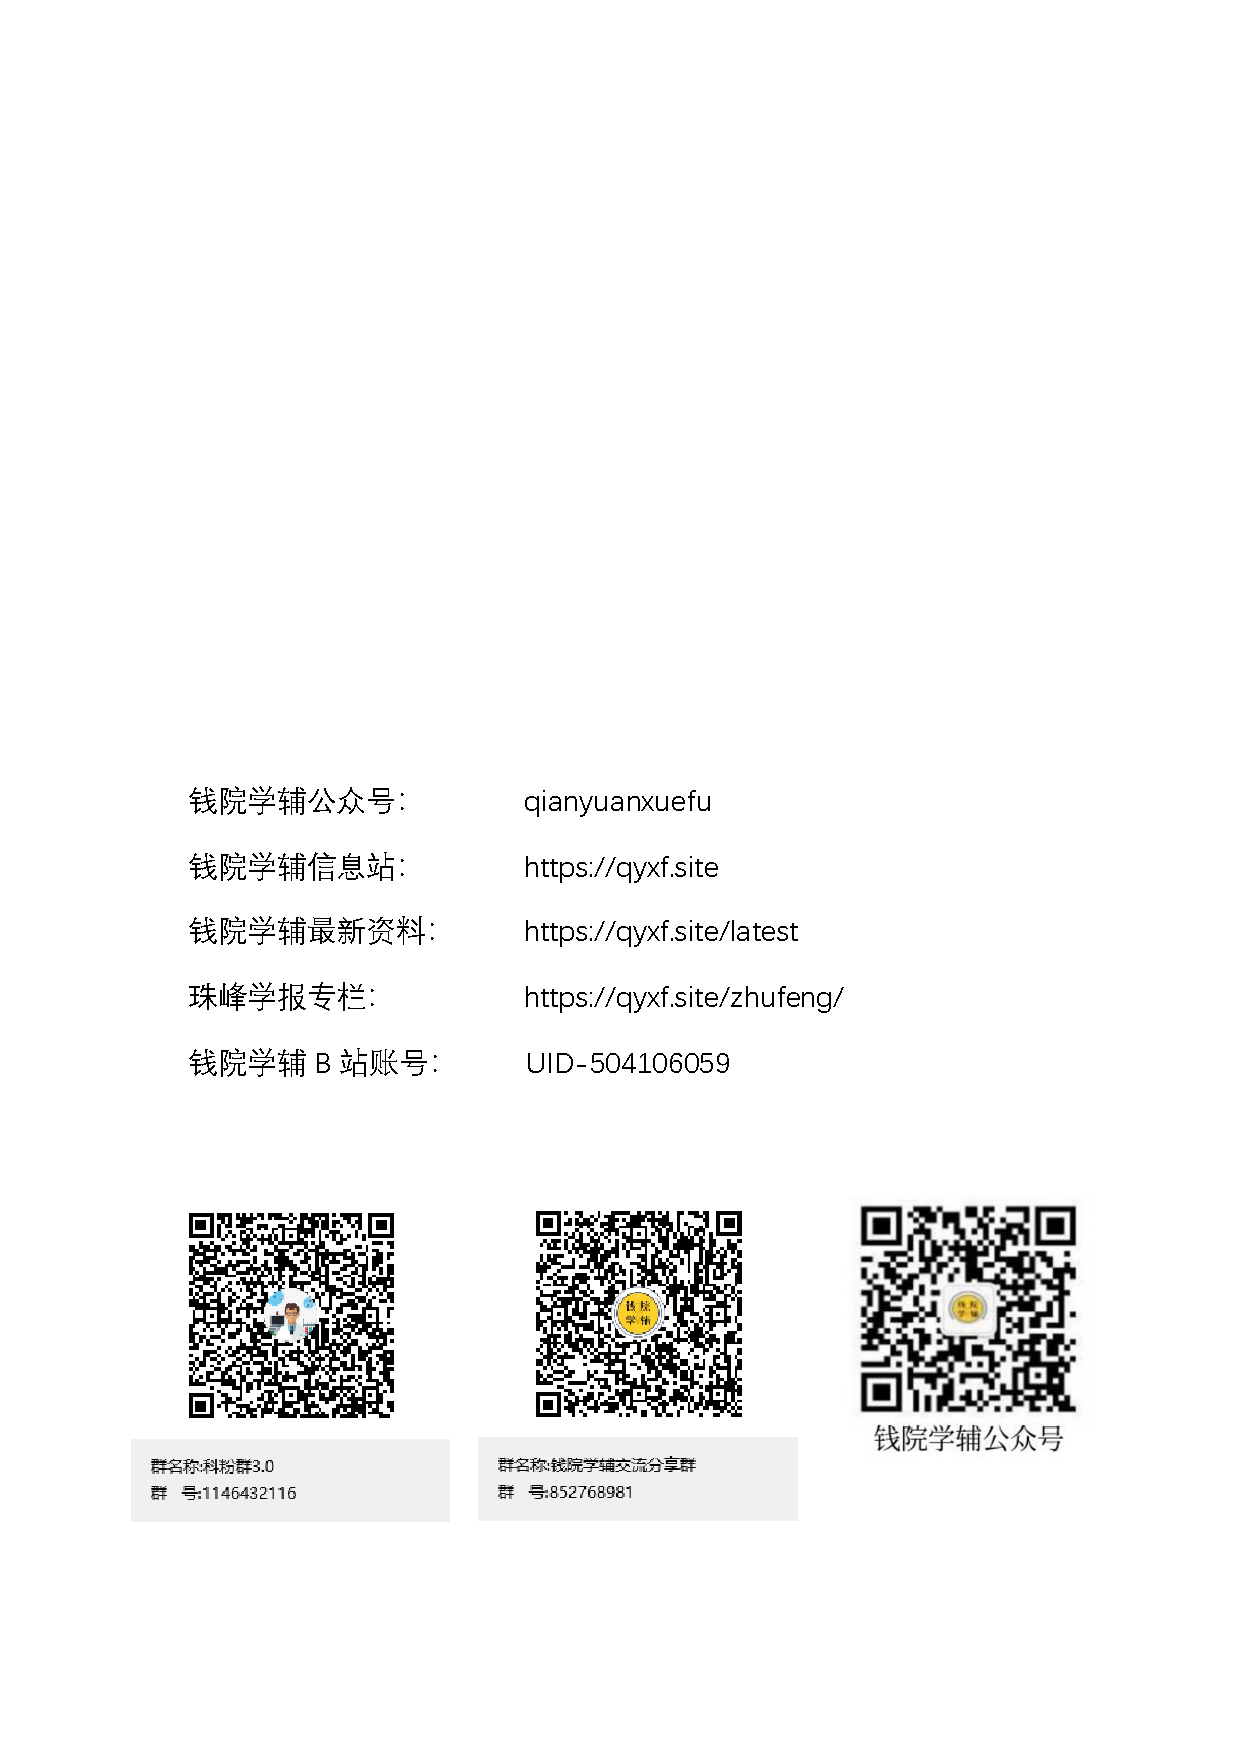
\includepdf[pagecommand = {\thispagestyle{empty}}, pages = - ]{lastpage.pdf}

\end{document}